\documentclass[10pt,a4paper]{report}
\usepackage[utf8]{inputenc}
\usepackage[russian]{babel}
\usepackage{amsmath}
\usepackage{amsfonts}
\usepackage{amssymb}
\usepackage{graphicx}
\author{Кенть Никита}
\title{Лабораторная работа №1.\\
	Программа для шифрования и подписи GPG, пакет Gpg4win}
\begin{document}
	\maketitle
	\tableofcontents
	\pagebreak
	
	\chapter{Цель работы}
	Научиться создавать сертификаты, шифровать файлы и ставить ЭЦП.
	\chapter{Описание лабораторной работы}
	Электронная цифровая подпись (ЭЦП) — реквизит электронного документа, полученный в результате криптографического преобразования информации с использованием закрытого ключа подписи и позволяющий проверить отсутствие искажения информации в электронном документе с момента формирования подписи (целостность), принадлежность подписи владельцу сертификата ключа подписи (авторство), а в случае успешной проверки подтвердить факт подписания электронного документа (неотказуемость).
	
	\chapter{Ход работы}
	\section{Создание ключевой пары OpenPGP}
	Запускаем \textbf{"Kleopatra"} и видим главное окно программы, в котором отображаются известные программе ключи (свои и чужие). Ключи в программе называются сертификатами. Чтобы создать новую ключевую пару, выбираем пункт меню \textit{"File -> New Certificate"} и выбираем формат OpenPGP. 
	
\begin{figure}[ht]	
	\center{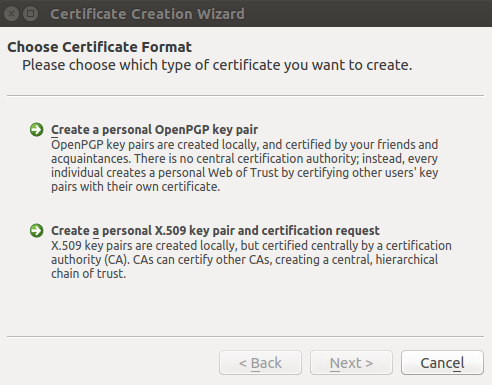
\includegraphics[width=0.8\linewidth]{pics/pic0}}
	\caption{Выбор формата сертификата}
	\label{pic:pic0}
\end{figure} 

Выбираем первый пункт (\textit{Create a personal OpenPGP key pair}). Открывается окно ввода информации о пользователе (Рисунок \ref{pic:pic1}).
	
\begin{figure}[h]
	\center{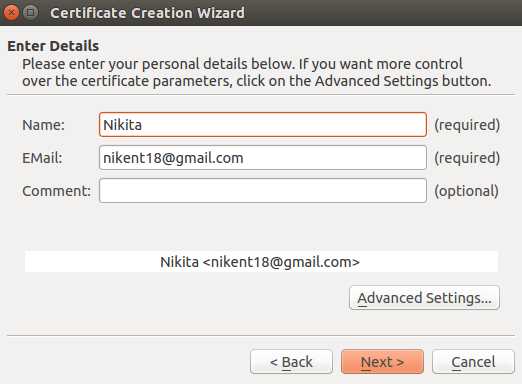
\includegraphics[width=1\linewidth]{pics/pic1}}
	\caption{Персональные данные}
	\label{pic:pic1}
\end{figure}

В итоге мы получаем готовый сертификат. Подробная информация о сертификате представлена на рисинке \ref{pic:pic2}

\begin{figure}[h]
	\center{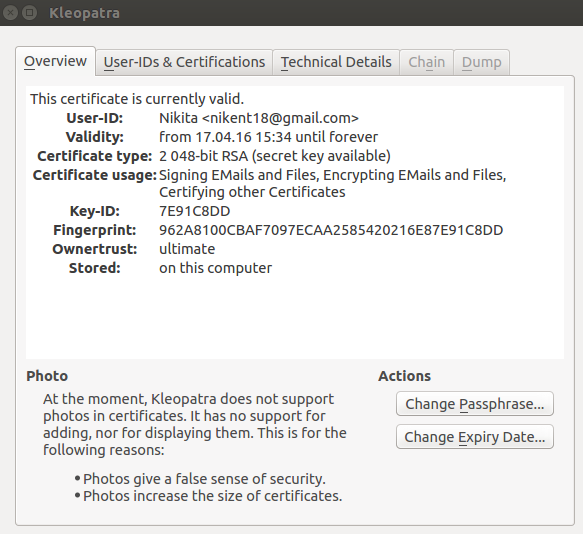
\includegraphics[width=1\linewidth]{pics/pic2}}
	\caption{Подробная информация о сертификате}
	\label{pic:pic2}
\end{figure}
\section{Экспорт сертификата}
Выполним экспорт сертификата.
Выполним команду \textit{"File ->  Export Certificate"}, в результате чего получим файл с расширением .asc. Содержание файла:
-----BEGIN PGP PUBLIC KEY BLOCK-----
Version: GnuPG v2.0.22 (GNU/Linux)

mQENBFcTgr8BCAC1DqAVqEy2GGrY5GpPuxiV83SYgv388YyUD99hFlwSSTHzOq22
jkr8N26BJcUlKgtr0iJVSZLBvI5cDTB5mFuUw9akbdcXUhXyE8OMVoPM7d4kjxGi
8JlHro7pamDztu72C7PMyI7JrSLKrCoFK0RiYI9F0sNuBzTw201zCEeGLa4dUMCA
+djOJAraSdT8bOWjQOuMfYnt1iT2A9aT7qnUwbG2D6bsCYkf0DkqpEUKW30JVQeL
D6AJXk0q/tY0cSRw9oZkXejxCYkaAHNUq1sO4mCNG0JCzPGYo7FoDkKec531Cfi6
ibAN9QlZOdnEyc3Tfo/y7xyzyVib5oftfwQ9ABEBAAG0G05pa2l0YSA8bmlrZW50
MThAZ21haWwuY29tPokBOQQTAQIAIwUCVxOCvwIbDwcLCQgHAwIBBhUIAgkKCwQW
AgMBAh4BAheAAAoJEEICFuh+kcjdfX8H/iVSbFwJzG9QR1Pk8Y36kjtRKY+zUcG1
g76auU/VZ/7OadgvsInKmI92kGwjvk8NThAeiVYM2H++slgUAWCH2RMwUFlVKKAe
RIW9WesERwMqwLT5x2YclwIa6sa97kvLzJgcwiWDhsy566EGfQXYPiiObe+E7gus
Q8lbtnELpFth2D8ggfNFaeC3/kDgWwA1nyQpELselM5WW+GIyYA8N/jt8fGJs6cb
raus4y9yA7vn2mmAjpdQ6ZHaT7zm3ktkNz7HNRspWbQhwngLTQuC7ml9adMMjJLF
gpRV+48ldRB7CKMQ/AW8Qdej75+as7A+iFRUskLvIFaAZtVvSt1DCYs=
=E+kT
-----END PGP PUBLIC KEY BLOCK-----

\section{Постановка ЭЦП на файл}
Для постановки ЭЦП на файл, требуется выполнить следующие действия:
 Выбрать пункт меню \textit{"File -> Sign/Encrypt Files"}, затем выбрать файл для шифрования и в появившемся окне выбрать действия, которые требуется выполнить

Этапы постановки ЭЦП изображены на рис. \ref{pic:pic3}, \ref{pic:pic4}, \ref{pic:pic5}

\begin{figure}[h]
	\center{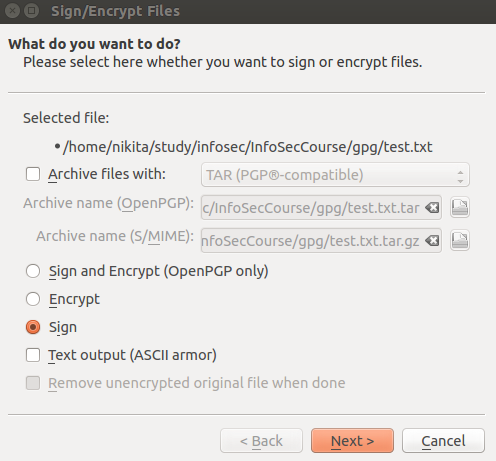
\includegraphics[width=1\linewidth]{pics/pic3}}
	\caption{Постановка ЭЦП шаг 1}
	\label{pic:pic3}
\end{figure}

\begin{figure}[h]
	\center{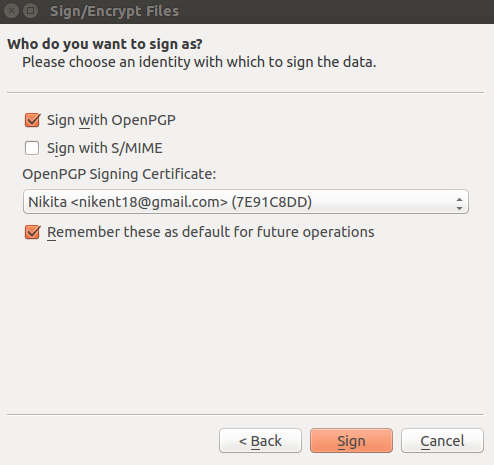
\includegraphics[width=1\linewidth]{pics/pic4}}
	\caption{Постановка ЭЦП шаг 2}
	\label{pic:pic4}
\end{figure}

\begin{figure}[h]
	\center{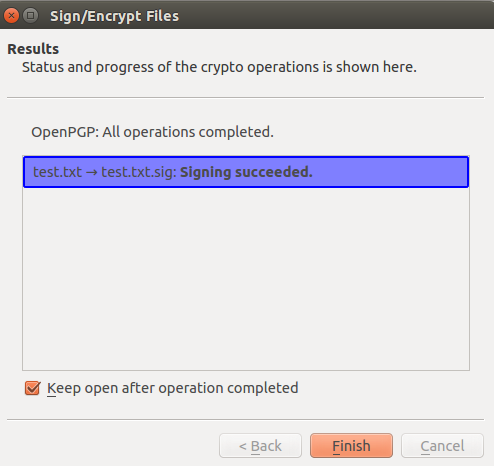
\includegraphics[width=1\linewidth]{pics/pic5}}
	\caption{Постановка ЭЦП шаг 3}
	\label{pic:pic5}
\end{figure}

В итоге появляется файл с названием test.txt.sig.



\section{Шифрование для коллеги}
Возьмем чужой сертификат (Рис. \ref{pic:pic6})

\begin{figure}[h]
	\center{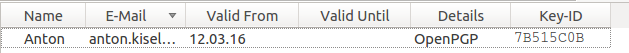
\includegraphics[width=1\linewidth]{pics/pic6}}
	\caption{Чужой сертификат}
	\label{pic:pic6}
\end{figure}

Выберем файл, зашифруем и подпишем его ЭЦП.\\

\begin{figure}[h]
	\center{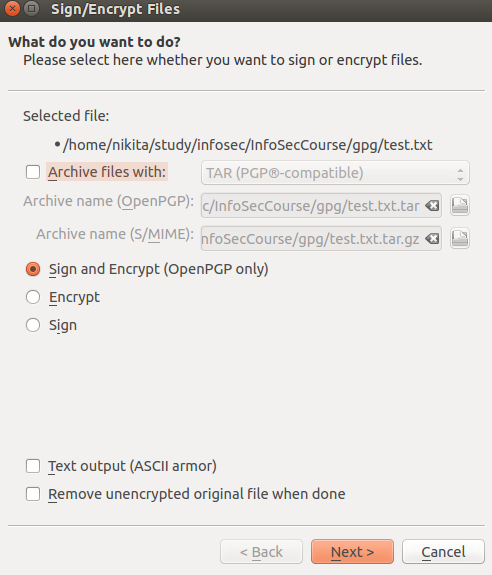
\includegraphics[width=1\linewidth]{pics/pic7}}
	\caption{Шифрование и установка ЭЦП}
	\label{pic:pic7}
\end{figure}	
Выберем для кого

\begin{figure}[h]
	\center{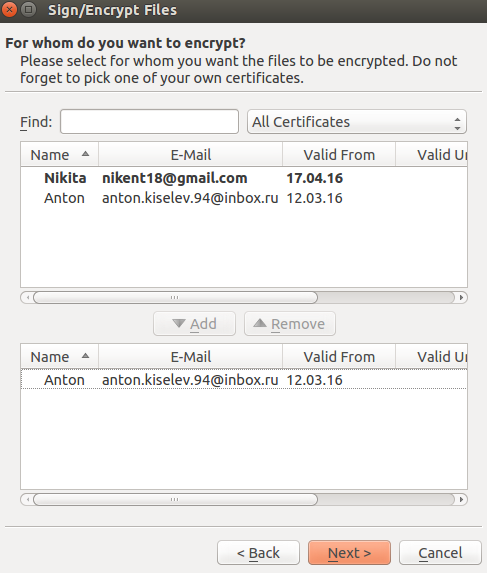
\includegraphics[width=1\linewidth]{pics/pic8}}
	\caption{Выбор для кого шифруем}
	\label{pic:pic8}
\end{figure}	

\begin{figure}[h]
	\center{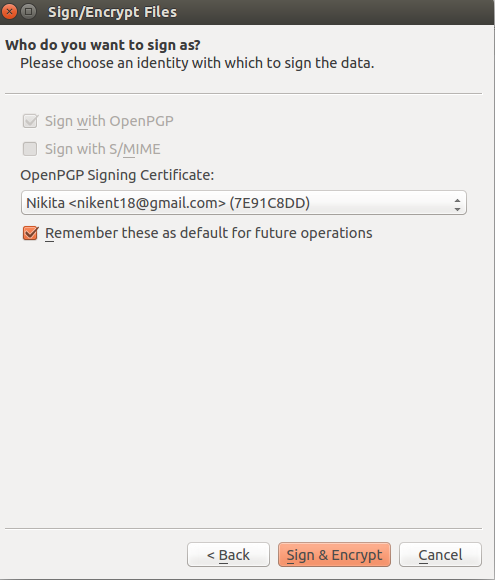
\includegraphics[width=1\linewidth]{pics/pic9}}
	\caption{Выбор идентификатора для ЭЦП}
	\label{pic:pic9}
\end{figure}	


\begin{figure}[h]
	\center{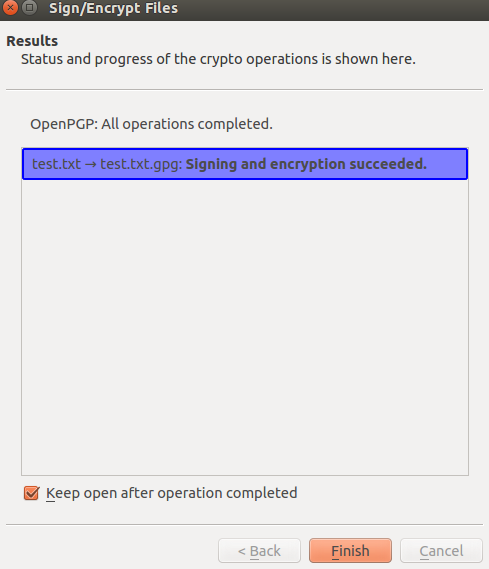
\includegraphics[width=1\linewidth]{pics/pic10}}
	\caption{Результат подписи}
	\label{pic:pic10}
\end{figure}	


Полученный от коллеги файл, зашифрованный с помощью нашего открытого ключа. Можно расшифровать, используея наш секретный ключ. Для этого выбираем пункт меню \textit{File -> Decrypt/Verify Files}.

\section{GNU Privacy handbook}
ля создания ключевой пары введем в консоле команду \textit{gpg2 --gen-key} И последуем пунктам, указанным в терминале
\begin{verbatim}
gpg: ВНИМАНИЕ: небезопасные права доступа у каталога содержащего файл конфигурации `/home/nikita/.gnupg/gpg.conf'
gpg (GnuPG) 2.0.22; Copyright (C) 2013 Free Software Foundation, Inc.
This is free software: you are free to change and redistribute it.
There is NO WARRANTY, to the extent permitted by law.

Выберите требуемый тип ключа:
   (1) RSA и RSA (по умолчанию)
   (2) DSA и Elgamal
   (3) DSA (только для подписи)
   (4) RSA (только для подписи)
Ваш выбор (?-подробнее)? 1
ключи RSA могут иметь длину от 1024 до 4096 бит.
Какой размер ключа необходим? (2048) 
Запрашиваемый размер ключа 2048 бит
Выберите срок действия ключа.
         0 = без ограничения срока действительности
      <n>  = срок действительности n дней
      <n>w = срок действительности n недель
      <n>m = срок действительности n месяцев
      <n>y = срок действительности n лет
Ключ действителен до? (0) 0
Ключ не имеет ограничения срока действительности
Все верно? (y/N) y

GnuPG необходимо составить UserID в качестве идентификатора ключа.

Ваше настоящее имя: Nikita
Email-адрес: nikent18@gmail.com
Комментарий: Super commnt
Вы выбрали следующий User ID:
    "Nikita (Super commnt) <nikent18@gmail.com>"

Сменить (N)Имя, (C)Комментарий, (E)email-адрес или (O)Принять/(Q)Выход? O
Для защиты секретного ключа необходима фраза-пароль.

Необходимо сгенерировать много случайных чисел. Желательно, что бы Вы
выполняли некоторые другие активные действия (печать на клавиатуре, движения мышью,
обращения к дискам) в процессе генерации; это даст генератору
случайных чисел возможность получить лучшую энтропию.



Необходимо сгенерировать много случайных чисел. Желательно, что бы Вы
выполняли некоторые другие активные действия (печать на клавиатуре, движения мышью,
обращения к дискам) в процессе генерации; это даст генератору
случайных чисел возможность получить лучшую энтропию.
gpg: ключ EA14D6B0 помечен как абсолютно доверяемый.
открытый и закрытый ключи созданы и подписаны.

gpg: проверка таблицы доверий
gpg: 3 ограниченных необходимо, 1 выполненных необходимо, PGP модель доверия
gpg: глубина: 0  корректных:   2  подписанных:   0  доверия: 0-, 0q, 0n, 0m, 0f, 2u
pub   2048R/EA14D6B0 2016-04-17
      Отпечаток ключа = D877 0535 170F 2D39 1775  0AB6 966A 14DA EA14 D6B0
uid                  Nikita (Super commnt) <nikent18@gmail.com>
sub   2048R/A7FED662 2016-04-17
\end{verbatim}
Посмотрим список всех имеющихся сертификатов, командой \textit{gpg --list-key}.
\begin{verbatim}
gpg: ВНИМАНИЕ: небезопасные права доступа к каталогу содержащему файл конфигурации `/home/nikita/.gnupg/gpg.conf'
/home/nikita/.gnupg/pubring.gpg
-------------------------------
pub   2048R/7E91C8DD 2016-04-17
uid                  Nikita <nikent18@gmail.com>

pub   2048R/7B515C0B 2016-03-12
uid                  Anton <anton.kiselev.94@inbox.ru>
sub   2048R/300C3B8E 2016-03-12

pub   2048R/EA14D6B0 2016-04-17
uid                  Nikita (Super commnt) <nikent18@gmail.com>
sub   2048R/A7FED662 2016-04-17
\end{verbatim}


Шифрации и ЭЦП документа для другого пользователя :
\begin{verbatim}
nikita@nikita-HP-ProBook-4520s:~$ gpg2 -se -r "Anton" /home/nikita/study/infosec/InfoSecCourse/gpg/test.txt
gpg: ВНИМАНИЕ: небезопасные права доступа у каталога содержащего файл конфигурации `/home/nikita/.gnupg/gpg.conf'

Необходима фраза-пароль для доступа к секретному ключу пользователя: "Nikita <nikent18@gmail.com>"
2048-бит RSA ключ, ID 7E91C8DD, создан 2016-04-17

gpg: 300C3B8E: Нет свидетельств принадлежности данного ключа лицу указанному в User ID ключа

pub  2048R/300C3B8E 2016-03-12 Anton <anton.kiselev.94@inbox.ru>
 Отпечаток главного ключа: 40E7 71F6 8766 73C2 F1CA  EFEE 5F58 B364 7B51 5C0B
      Отпечаток подключа: 39F6 4CB9 91B8 78BE 02F8  9B87 CC57 9665 300C 3B8E

Нет уверенности принадлежности ключа человеку указанному
в User ID ключа.  Если ТОЧНО знаете, что делаете,
можете ответить на следующий вопрос утвердительно.
\end{verbatim}

Экспорт своего открытого ключа:
\begin{verbatim}
nikita@nikita-HP-ProBook-4520s:~$ gpg2 --armor --export nikent18@gmail.com
gpg: ВНИМАНИЕ: небезопасные права доступа у каталога содержащего файл конфигурации `/home/nikita/.gnupg/gpg.conf'
-----BEGIN PGP PUBLIC KEY BLOCK-----
Version: GnuPG v2.0.22 (GNU/Linux)

mQENBFcTgr8BCAC1DqAVqEy2GGrY5GpPuxiV83SYgv388YyUD99hFlwSSTHzOq22
jkr8N26BJcUlKgtr0iJVSZLBvI5cDTB5mFuUw9akbdcXUhXyE8OMVoPM7d4kjxGi
8JlHro7pamDztu72C7PMyI7JrSLKrCoFK0RiYI9F0sNuBzTw201zCEeGLa4dUMCA
+djOJAraSdT8bOWjQOuMfYnt1iT2A9aT7qnUwbG2D6bsCYkf0DkqpEUKW30JVQeL
D6AJXk0q/tY0cSRw9oZkXejxCYkaAHNUq1sO4mCNG0JCzPGYo7FoDkKec531Cfi6
ibAN9QlZOdnEyc3Tfo/y7xyzyVib5oftfwQ9ABEBAAG0G05pa2l0YSA8bmlrZW50
MThAZ21haWwuY29tPokBOQQTAQIAIwUCVxOCvwIbDwcLCQgHAwIBBhUIAgkKCwQW
AgMBAh4BAheAAAoJEEICFuh+kcjdfX8H/iVSbFwJzG9QR1Pk8Y36kjtRKY+zUcG1
g76auU/VZ/7OadgvsInKmI92kGwjvk8NThAeiVYM2H++slgUAWCH2RMwUFlVKKAe
RIW9WesERwMqwLT5x2YclwIa6sa97kvLzJgcwiWDhsy566EGfQXYPiiObe+E7gus
Q8lbtnELpFth2D8ggfNFaeC3/kDgWwA1nyQpELselM5WW+GIyYA8N/jt8fGJs6cb
raus4y9yA7vn2mmAjpdQ6ZHaT7zm3ktkNz7HNRspWbQhwngLTQuC7ml9adMMjJLF
gpRV+48ldRB7CKMQ/AW8Qdej75+as7A+iFRUskLvIFaAZtVvSt1DCYuZAQ0EVxO1
ewEIALmvwb/CiIJxsoHK2r+56UtBFp1W7NQju+HtDprbFxIbaLu0dqgR9pCpwEAP
NjEtHXi+jC1jnlWHv2hX/Z6C10U9fMITeaI4KEY3F/LajclffrX/V05RHiS3UppL
ySwRi89qR9abgahoVYUjIVBe/hZqM1+CYXoMg5Ud2iFs8MXj4+c7xDJJFQcICFbs
VK1dTwLgumd4yFYodTMxO7ppjkmz3mkfZ9z/ovmuC8dQCVMveqjatDz020C7W5hH
aIgi6bo1BE/i0H8qX39Ix3G4JvyfdU11SWoJHfxvMmQDNaI2Pb6ui94Zob3gdRwd
e/zefGHejeoUClYbiaPVqjzGZGEAEQEAAbQqTmlraXRhIChTdXBlciBjb21tbnQp
IDxuaWtlbnQxOEBnbWFpbC5jb20+iQE5BBMBAgAjBQJXE7V7AhsDBwsJCAcDAgEG
FQgCCQoLBBYCAwECHgECF4AACgkQlmoU2uoU1rAiVwgAqAemJSDaBcLmYtHmdyOH
Qt0HJQvRBpw0B3cnend/rcvN4BWPsSRQa4F0MUIwMXshHayKKfDMapHQydc8P9wB
AlukiBJnpR8xsO8cYK6Fu9010LCQMHpDiaAl5dPYwWjcLWfWULCLwwMLBFoil/N1
dMbF3tuVmxyoxlQ5h8qKcY1yN7grGIxicfVtdEzBZrmfipja8IFGFFuTPo0nWjS8
nZA5cqufGUiKgcLFOwdJvWh9YFzMem83JAsf8X1lAM2huQSWSGr9FTT7KRLxVn3o
d86Vfh1FyVxt1403ud9YM4QQCS8jBeXKYqHd3KkOSuqWwT+GtycyLmxDDMTP4zHR
0LkBDQRXE7V7AQgAoVH5YciyM/8oEtGh2TFGCGgPBgia+dSP8LuPOcckiSAUwGvF
3pn6TnNwJBMR7tH/XLE9Zij26S3/pgg+pX14K6gKqo2JXDPOqUx9uBBJ+o5EU1jf
K4nOyKgVRFjRGnpfsXGFzioatD2Y/dwVEk8HvnU+qQty2NevmdM8RB2S6jaFJnUP
H8pJ5714bKj8eqOHu0byfSCWK5zp+LCsI5gsQe2yxDFyesEVr/zaBBiTDt8ex9jM
khf5QUkYVr3erRwgsgkiWPNnwfGh5A+mnE8wd2phzlqRmJAN0SLf6rA5NLkv82cJ
hW4pwQI5/gfwi3Ml1inezfgEv6uRYeZUdARVHQARAQABiQEeBBgBAgAJBQJXE7V7
AhsMAAoJEJZqFNrqFNawsCoH9jdhdoKvtMEJNl8kowFsqEm1caN8mMdHz56vxAmH
/tT6kyCKZvgHMa4NhCLQhcEUaYzZLWOAlKvmtYYhCS1Q1Y5T+TU0pUD+5jNHA1uX
KiQJwsMf5hWVqnb3lS3faGeMlkWWU3RRuZTSj3cZwH+JN+lcIxzKo68zeYDo6/LV
xeW2++p0/0DtN8fT7yp1+/qalpMb5lQjJuSd+ZhnqiPDK1ogiH3sgPzfasH4nuAf
7w4gt6aiCxjQFeYqwjX4vmd9ejus+vI3sbcbrJ8I7AA2hIZAazfwa0KEvuv/y2wB
UCkHGQWS7gxsRgiCH/QXwIB1OX9roh7eHGteN9RY9dRaKA==
=DId+
-----END PGP PUBLIC KEY BLOCK-----
\end{verbatim}

\end{document}